\chapter{Context (Estat de l'art)}\label{C:compaginacio}

\section{Ús lliure de RF}
Amb l'establiment de les bandes ISM (Afegir referencia) es crea la possibilitat per el públic general utilitzar comunicació inal·làmbrica amb molta facilitat. Això es deu a que l'establiment de les bandes ISM està acceptat de manera (mes o menys(?)) de la mateixa manera internacionalment.
Això facilita el disseny de productes per al consumidor habitual que ràpidament veu els avantatges de la comunicació inal·làmbrica entre dispositius.
En aquest entorn sorgeix la necessitat d'establir estandards entre le companyies principals dels sectors. Per definir els estandards s'agrupen les companyies i formen grups com al WIFI Alliance o ...

\subsection{Wifi}
La tecnologia de comunicació més popular avui en dia és la WIFI, dissenyada originalment als anys (?) i establerta als anys (?) orientada a permetre una connexió (* bona) i sense consideració per les interferències entre si mateixa que no es podien preveure llavors.  
- Avantatges
- Innovació
- Evolució

\subsection{Bluetooth Classic}
Bluetooth enlloc de estar orientat a donar connexió a internet estava orientat a connectar dispositius entre si (punt a punt) per a la transferència de fitxers com contactes o fotografies.
Posteriorment es va poder aconseguir velocitats suficients pel \textit{streaming} de música en temps real.
Junt amb l'arribada dels telèfons intel·ligents els auriculars inal·làmbrics es van fer populars i també es va establir la dominància de bluetooth per a escoltar música sense cables.
Amb aquest objectiu es va millorar bluetooth per tal de ser més resistent a interferències i a poder transmetre més velocitat per poder transmetre música d'alta fidelitat.
Per un altre costat però va començar a sorgir el Internet of Things, basat en tenir molts dispositius connectats i això va generar necessitats que no es podien cobrir amb les tecnologies desenvolupades anteriorment.

\section{MANETS}
Bluetooth classic no permetia ni tenir més d'una connexió establerta amb dispositius i l'arquitectura feia que s'utilitzés bastanta energia per establir i mantenir una connexió encara que es volguessin transmetre molt poques dades.
Aquestes limitacions feien que fos necessari definir nous protocols que estiguessin orientats a connexions de poques dades cap a més d'un dispositiu i que utilitzessin el mínim de energia possible.

\subsection{BLE}
Bluetooth Low Energy no té cap relació amb Bluetooth Classic pel que fa a l'arquitectura del protocol. Tot i compartir nom (perque?) queda clar que no estem parlant del mateix amb el simple fet que no son compatibles entre sí. Tot i així comparteixen l'ús de la banda freqüencial de 2,4 GHz igual que altres protocols sense fils. Al 2016 es va anunciar la versió 5.0 anomenada Bluetooth 5 (sense el punt)[cita] i se li va canviar el nom (aclariment).

% Diferencies entre classic i low energy

\subsection{Altres Protocols}
Bluetooth Low Energy no és l'únic protocol orientat a la connexió de dispositius amb baix consum energètic. També existeixen els següents protocols:
Zigbee, utilitzat en Philips Hue
Zwave Ring (home security)
6lowpan
insteon
lorawan

% Prodcutes que utilitzen cadascun

\subsection{Comparació}
Tot i que els protocols tenen molt en comú cada un es diferencia de la resta en els detalls, a continuació veiem una comparació de les capacitats de cada un dels protocols

\section{BLE Stack}
Un cop vistes les característiques generals del protocol cal entendre com funciona per dins.
En entrar en detall queda clar com el protocol s'ha dissenyat de forma molt flexible 

\begin{figure}[h!]
	\begin{center}
		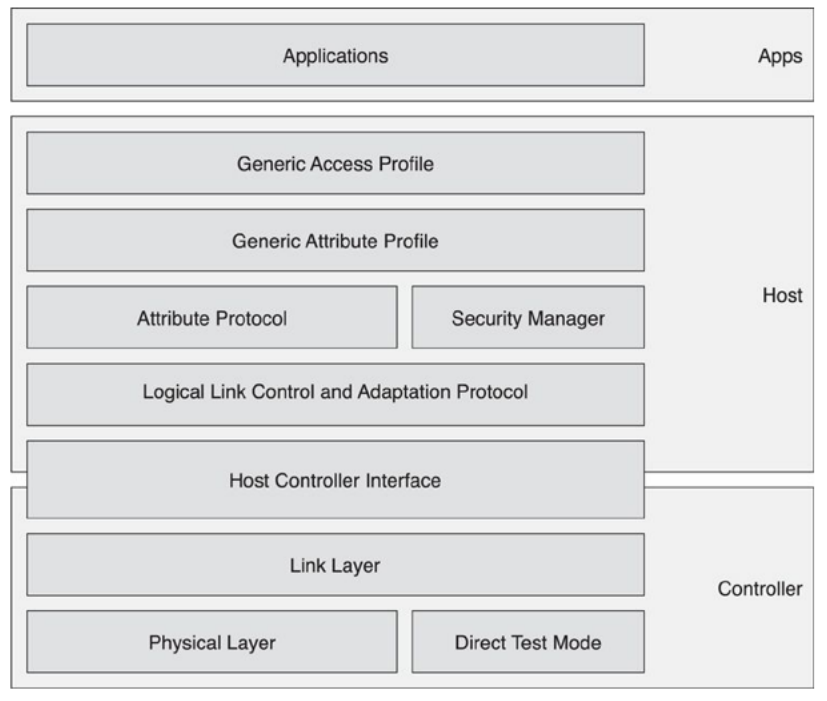
\includegraphics[width=0.6\textwidth]{./images/BLE_Stack.png}
		\caption{Pila de BLE \cite{ble_stack}}
		\label{ble_stack}
	\end{center}
\end{figure}

La pila pròpia de Bluetooth Low Energy esta dividida en dues parts, el controladors i el \textit{host}. Aquestes dues parts són independents i utilitzen el protocol HCI (\textit{Host Controller Interface}) per comunicar-se entre si. Aquest protocol pot estar implementat amb qualsevol protocol de transport físic com USB o UART. També hi ha la possibilitat d'implementar les dues parts en un mateix xip. L'arquitectura de si està implementat amb un o dos components s'anomena configuració de xip únic o dual.


\subsection{Controller}
El controlador compren la capa física i la capa d'enllaç.

\subsubsection{PHY}
La capa física és la que s'encarrega de la comunicació anal·lògica modulant i desmodulant les senyals.
Tal i com ja s'ha comentat abans treballa a la banda de 2.4 GHz en 40 canals diferents

\begin{figure}[h!]
	\begin{center}
		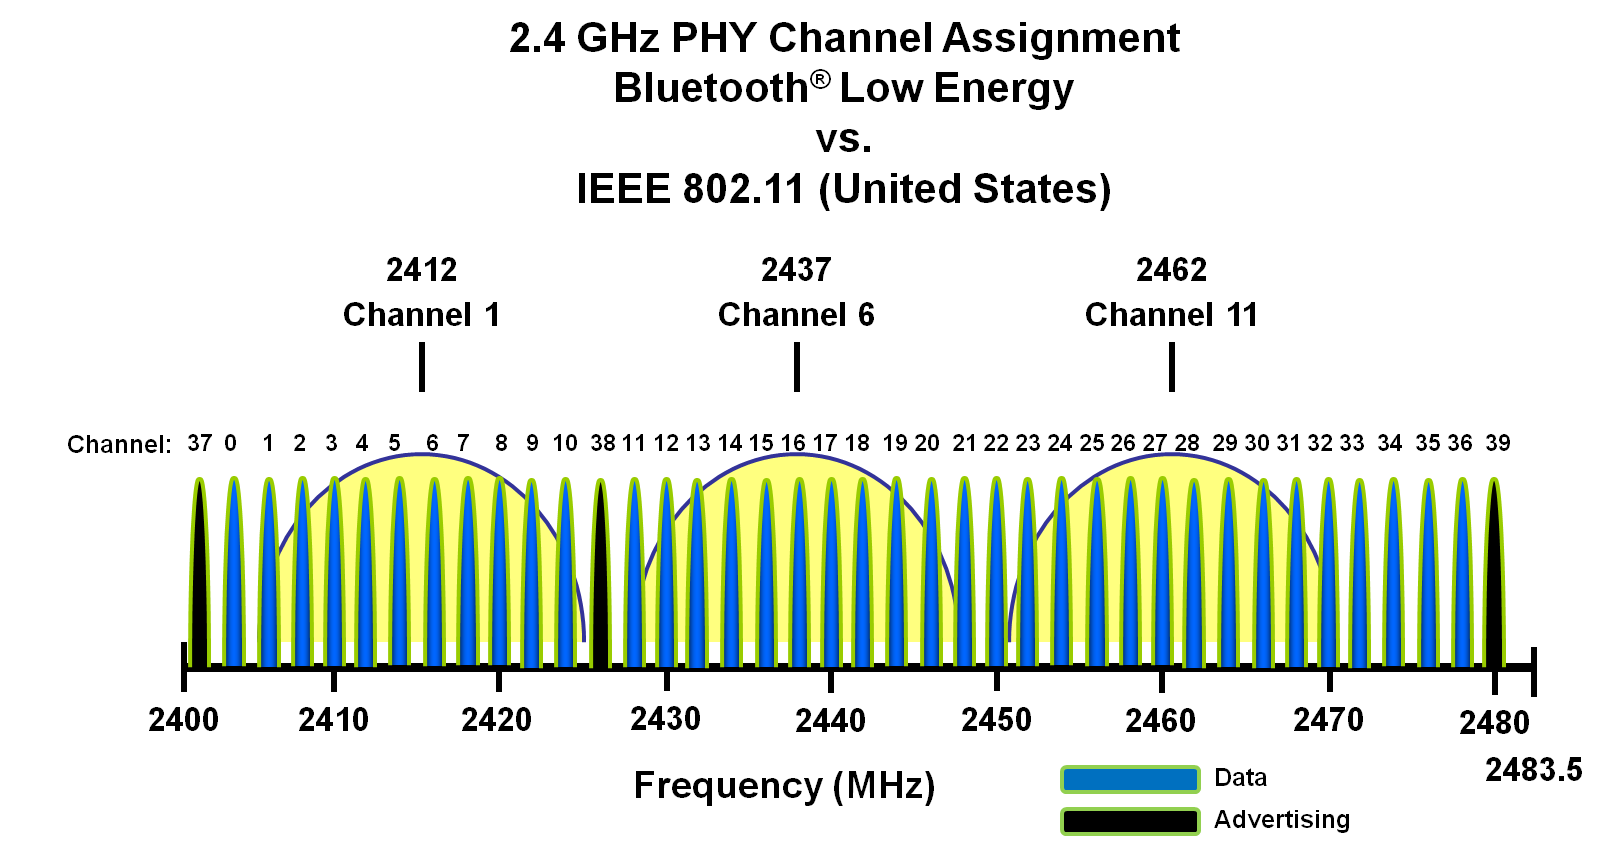
\includegraphics[width=0.8\textwidth]{./images/ble_channel_assignment.png}
		\caption{Pila de BLE \cite{ble_stack}}
		\label{ble_stack}
	\end{center}
\end{figure}

Els canals es classifiquen com a dades o d'anunci (\textit{Advertisment}). Els canals d'advertisment que són els que es vol tenir més qualitat coincideixen en els espais freqüencials que minimitzen les interferències amb els canals wifi més comuns (1, 6 i 11).

Tot i que amb aquest protocol l'objectiu és transmetre poca informació de forma eficient, es per això que, tot i estar tractant amb paquets d'informació molt curts cal una tassa de transmissió el més alta possible. D'aquesta manera s'aconsegueix que les radio tant del transmissor com la dels receptors estiguin el mínim temps possible actives.
La tassa de transmissió física del protocol es de 1 Mbps per a BLE 4 que augmenta opcionalment a la versió 5 a 2 Mbps.
La modulaci

Pel que fa a la potencia de transmisió es pot controlar de tal manera que si és necessari i no limita la comunicació es pot disminuir per gastar menys energia. Tot i així, en el paquets que s'envien es menciona la potència amb la que s'ha transmès per a que el receptor pugui estimar la distància fins al transmisor(?).

La modulació utilitzada per BLE és la mateixa que pel IEEE 802.11, GFSK (\textit{Gaussian Frequency Shift Keying}). Aquesta modulació és una de les més robustes, simples d'implementar i és el que permet (en part) a BLE tenir un abast molt més gran que Bluetooth Clàssic. Aplicar el filtre gaussià és útil ja que permet reduir el consum pic de energia \cite{BLE_Review} i també redueix les interferències en freqüències veïnes.


\subsubsection{Link Layer}

La capa d'enllaç és la encarregada de escanejar, anunciar i gestionar connexions amb altres dispositius

Per mitigar l'efecte de les interferències el protocol utilitza salts en freqüència (\textit{frequency hopping}). Això permet reduir l'impacte d'una interferència estreta (?). Els salts són de entre 5 i 16 canals d'entre els 37 dedicats a dades.

Bluetooth també permet la implementació de salts en freqüència adaptatius on només s'utilitzen canals suficientment bons descartant aquells en que es considera que hi ha masses interferències.

\subsection{Host}
\subsubsection{L2CAP}
La \textit{Logical Link Control and Adaptation Protocol} és la capa encarregada de l'establiment de la connexió lògica, multiplexament de protocols, segmentació i 'reasembly', control de flux per cada canal L2CAP.

La multiplexació de protocols és necessària tal que serveix per identificar quin és el protocol que s'utilitza en les capes superiors.

Per limitació física de l'arquitectura existeix una MTU (\textit{Maximum Transmission Unit}) i per tant els paquets de les capes superiors es converteixen en paquets més petits per a les capes inferiors.
Aquesta MTU es pot definir per cada connexió així flexibilitzant la varietat de dispositius amb els que es pot connectar un mateix dispositiu.

QOS Aquesta capa també és la que fa el seguiment de la qualitat de la connexió i dels recursos utilitzats per assegurar-se que les necessitats dels serveis es compleixen.

\subsubsection{SMP}
La capa \textit{Security Management Protocol} proveeix de diferents serveis relacionats amb la seguretat de la connexió.
Aquests serveis són: autenticació i autorització de dispositius i també integritat, confidencialitat i privacitat de les dades.
El protocol té tipus d'emparellament i generació de claus flexible per aconseguir reduir els requeriments de memòria i energia.

\subsubsection{ATT \& GATT}
El \textit{Attribute Protocol} és el protocol d'aplicació més comú per a BLE i el \textit{Generic Attribute Profile} defineix com utilitzar el protocol per oferir serveis a capes superiors.
El ATT és un protocol dissenyat per a dispositius \textit{Low Energy} amb l'objectiu de minimitzar la quantitat de dades transmeses. El atribut està format per 4 elements, \textit{handle}, UUID, permisos  i \textit{value}.

El \textit{handle} fa la distinció única entre els diferents atributs, ocupa 16 bits i no és obligatori que siguin valors seqüencials. És molt útil ja que s'utilitza per referenciar el atribut amb el mínim de bits possibles.
El UUID (\textit{Universal Unique IDentifier}) identifica el tipus d'atribut, aquest numero pot ser de 16 bits si s'utilitza algun que ja estandarditzat pel SIG o bé en tindrà 128 bits si està definit pel fabricant.
En els permisos s'indicarà quin tipus d'accés té el client a la informació (només lectura, lectura i escriptura ...). També pot estar definit si requereix un nivell mínim d'encriptació o si es necessari l'autenticació.
Per últim el valor del atribut serà on hi ha la informació en si i la seva longitud i interpretació dependrà del UUID tot i que té un limit de 512 bytes.

Des del punt de vista del protocol els dispositius són clients i servidors, normalment el client pren la iniciativa demanant dades però el servidor també te la capacitat d'iniciar una comunicació per exemple notificant quan un valor ha canviat.

La definició del ATT és massa genèrica per si sola tal que seria comú que per fer el mateix es desenvolupessin múltiples definicions que fossin incompatibles entre sí.
Per tal de tenir millor definits els serveis s'utilitza el GATT. El GATT permet definir perfils que agrupen múltiples atributs en un sol servei \cite{services}.

\begin{figure}[h!]
	\begin{center}
		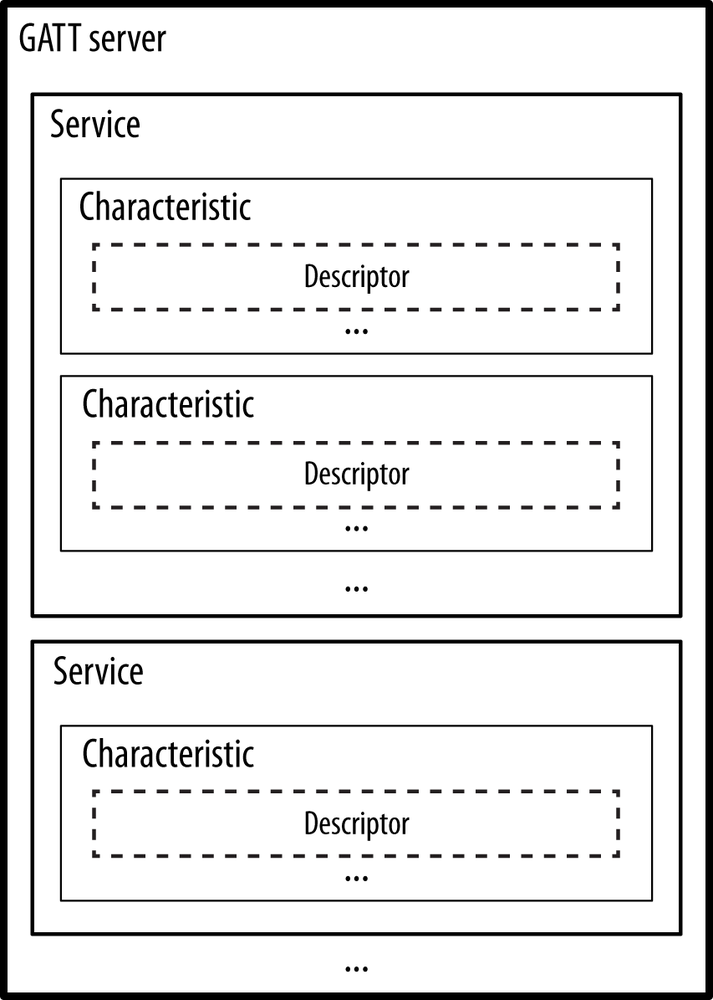
\includegraphics[width=0.3\textwidth]{./images/GATT_Hierarchy.png}
		\caption{Jerarquia de GATT \cite{GATT_Hierarchy}}
	\end{center}
\end{figure}

En un llistat de atributs el GATT identifica els serveis tenint en compte que cada servei comença amb un atribut amb el UUID 0x2800, els següents atributs formaran part del mateix servei fins que es trobi un nou atribut amb UUID 0x2800. En el valor del atribut on es defineix el servei (UUID 0x2800) hi ha un altre UUID que especifica quin tipus de servei és.

Cada servei té característiques \cite{characteristics} que s'identifiquen perquè el UUID és 0x2803, en aquests atributs en el seu valor hi haurà un nou UUID que identifica la informació que es troba en el atribut amb un cert \textit{handle} que també estarà indicat.

\begin{center}
	\begin{tabular}{|l|l|l|l|}
		\hline
		Handle	&	UUID	&	Descripció						&	Valor		\\ 	\hline
		0x0100	&	0x2800	&	Battery Service					&	UUID 0x180F	\\		\hline
		0x0101	&	0x2803	&	Characteristic: Battery Level	&	\parbox[t]{4cm}{UUID 0x2A19	\\ Value handle: 0x0102}	\\	\hline
		0x0102	&	0x2A2B	&	Battery Value					&	20	\\	\hline
		0x0103	&	0x2800	&	Custom Temperature Service		&	UUID 	706676c8-3e49...	\\	\hline
		0x0104	&	0x2803	&	Characteristic: Temperature		&	\parbox[t]{4cm}{UUID 0x2A6E	\\ Value handle: 0x0105}	\\		\hline
		0x0105	&	0x2A6E	&	Temperature Value				&	25.45	\\	\hline
		0x0106	&	0x2803	&	Characteristic: date/time		&	\parbox[t]{4cm}{UUID 0x2A08	\\ Value handle: 0x0107}	\\		\hline
		0x0107	&	0x2A08	&	Date/Time						&	1/1/1980 12:00	\\
		\hline
	\end{tabular}

Exemple de possibles atributs
\end{center}

En aquest exemple es pot veure que tenim 2 serveis diferents ja que hi ha 2 UUIDs 0x2800 i tenim 3 característiques en total (una pel primer servei i dues pel segon) ja que hi ha 3 atributs amb UUID 0x2803.
Com que els calors corresponents al nivell de bateria i la temperatura estan estandarditzats no cal especificar a que es refereixen a percentatge de bateria restant i a graus Celsius.

Es pot veure com el servei que està definit per a la temperatura no forma part de l'estàndard ja que té 128 bits. El número que s'ha escollit és un UUID completament aleatori: 706676c8-3e49-4ecc-9379-fa9851444e53. Tot i que no hi ha una coordinació per assegurar-se que diferents desenvolupadors no utilitzen el mateix UUID degut a la longitud (128 bits) es considera improbable. La condició que ha de complir el UUID és que no sigui XXXXXXXX-0000-1000-8000-00805F9B34FB ja que aquest sufix correspon als que estan reservats per a l'estandard. En cas de voler tenir un UUID global reservat es pot fer pagant \$2.500 i també es poden veure tots els que ja s'han reservat per a empreses a questa web \cite{reservedUUIDs}.

En aquest exemple no n'hi ha cap però les característiques poden tenir descriptors \cite{descriptors} que permeten aportar informació addicional sobre la característica que els precedeix.

\subsubsection{GAP}
En quant es realitza una connexió els dispositius han de definir-se entre els següents rols: Anunciador (\textit{Advertiser}) o Escàner (\textit{Scanner}), Esclau (\textit{Slave}) o Mestre (\textit{Master}) i Emissor (\textit{Broadcaster}) o Observador (\textit{Observer}).
Aquests rols són independents per cada connexió per tant un dispositiu pot ser mestre en una connexió i alhora esclau en una altre.

Per iniciar una connexió entre dos dispositius (\textit{Peer-to-Peer}) un dispositiu vol ser descobert i envia missatges anunciant-se. L'altre dispositiu, que es vol connectar passa a ser un escàner. Aquest envia un paquet amb el requeriment de connexió, un cop acceptat, el dispositiu que fa d'escàner passa a ser mestre i el que anunciava passa a ser esclau.

També és possible transmetre informació des d'un dispositiu a tots aquells que estiguin escoltant, per tant, una comunicació de un a molts (\textit{One-to-many}). En aquest cas aquell que vol transmetre informació és el emissor i els dispositius que escolten són observadors.

\begin{figure}[h]
	\begin{center}
		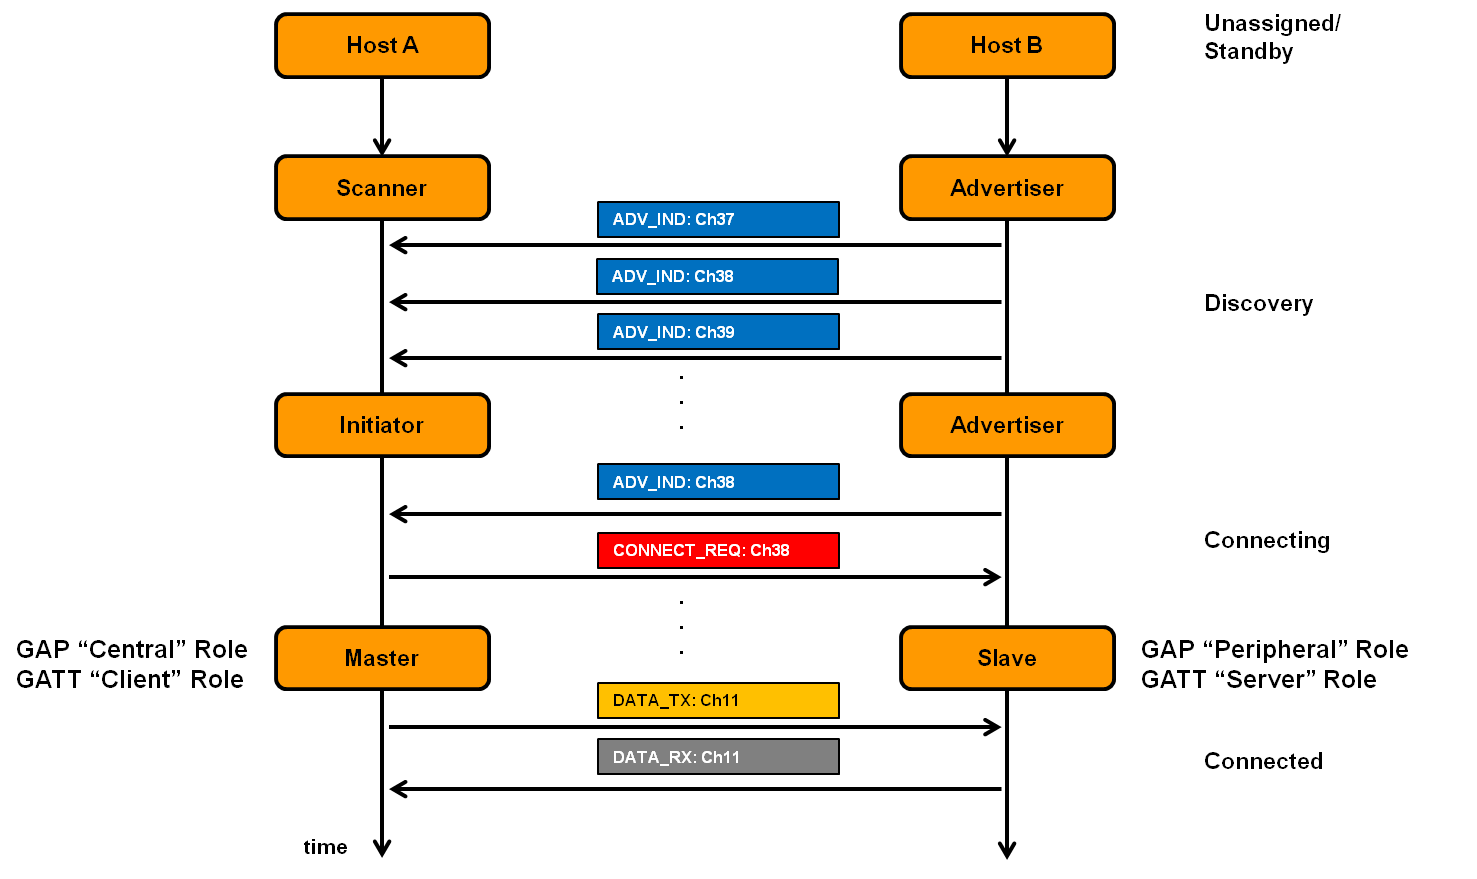
\includegraphics[width=1\textwidth]{./images/rols_unicast.png}
		\caption{Pila de BLE \cite{ble_stack}}
		\label{ble_stack}
	\end{center}
\end{figure}

